\documentclass[12pt,a4paper,oneside,brazil]{abntex2}
\usepackage[utf8]{inputenc}
\usepackage[T1]{fontenc}
\usepackage[brazil]{babel}
\usepackage{graphicx}
\usepackage{lipsum} % Pacote para gerar texto fictício
\usepackage{helvet}
\usepackage{ragged2e}

\renewcommand{\familydefault}{\sfdefault}

\titulo{PLATAFORMA DE EDIÇÃO/AUTOMAÇÃO PARA TRABALHOS ACADÊMICOS}
\autor{HIGOR FERREIRA ALVES SANTOS}
\orientador{Nome do Orientador}
\instituicao{%
    PONTIFÍCIA UNIVERSIDADE CATÓLICA DE GOIÁS
    \par
    ESCOLA POLITÉCNICA E DE ARTES
    \par
    ENGENHARIA DE COMPUTAÇÃO
    }
\local{GOIÂNIA - GO}
\data{2023}

% Início do documento
\begin{document}

% Capa personalizada
\begin{capa}
    \center

    \OnehalfSpacing
    \ABNTEXchapterfont\bfseries\textsc{\imprimirinstituicao}

    \vfill

    % Incluir logotipo
    
\includegraphics[width=0.15\textwidth]{./src/assets/logo.png}

    \vfill

    \ABNTEXchapterfont\bfseries\imprimirtitulo

    \vfill

    \imprimirautor

    \vfill

    \bfseries\imprimirlocal

    \bfseries\imprimirdata
\end{capa}

% Folha de rosto personalizada
\begin{folhaderosto}

    \centering

    \imprimirautor

    \vfill

    \ABNTEXchapterfont\bfseries\imprimirtitulo

    \vfill

    % \justifying
    % \noindent\hspace*{70mm}%
    % \begin{minipage}{\dimexpr\textwidth-70mm}
    %     \textnormal{Trabalho de Conclusão de Curso apresentado à
    %     Escola Politécnica e de Artes, da Pontifícia
    %     Universidade Católica de Goiás, como parte dos
    %     requisitos para a obtenção do título de Bacharel em
    %     Engenharia de Computação.% \\

    %     Orientador:\\
    %     \begin{flushright}
    %         Prof. M.E.E. Marcelo Antônio Hadad\\
    %     \end{flushright}
    %     Banca examinadora:\\
    %     \begin{flushright}
    %         Nome1\\
    %         Nome2\\
    %     \end{flushright}
    %     }
    % \end{minipage}

    % \vfill

    % \centering

    \bfseries\imprimirlocal

    \bfseries\imprimirdata
\end{folhaderosto}

% Folha de aprovação
\clearpage
    \centering
    \imprimirautor

    \vfill

    \ABNTEXchapterfont\bfseries\imprimirtitulo

    \vfill

    \justifying

    \textnormal{Trabalho de Conclusão de Curso aprovado em sua forma final pela Escola Politécnica e de
    Artes, da Pontifícia Universidade Católica de Goiás, para obtenção do título de Bacharel em
    Engenharia de Computação, em: \_\_\_/ \_\_\_/ \_\_\_\_\_}

    \centering

    \vspace*{3cm}

    \begin{flushright}
    \rule{10cm}{0.4pt}\\
    \textnormal{Orientador: Prof. M.E.E. Marcelo Antônio Hadad}

    \vspace*{10mm}

    \rule{10cm}{0.4pt}\\
    \textnormal{Orientador1:}

    \vspace*{10mm}

    \rule{10cm}{0.4pt}\\
    \textnormal{Orientador2:}
    \end{flushright}

    \vspace*{6cm}

    \bfseries\imprimirlocal

    \bfseries\imprimirdata
\clearpage % Começa uma nova página para a folha de rosto

% Correção: Usar \tableofcontents para o Sumário
\tableofcontents
\listoffigures   % Lista de Figuras
\listoftables    % Lista de Tabelas

\textual

\chapter{Introdução}
Este é um exemplo de texto com uma nota de rodapé.\footnote{Aqui está o texto da nota de rodapé.} \lipsum[1]

\section{Subtítulo de Nível 1}
Texto com outra nota de rodapé.\footnote{Outro exemplo de nota de rodapé.} \lipsum[2-3]

\subsection{Subtítulo de Nível 2}
\lipsum[4]
\subsubsection{Subtítulo de Nível 3}
\lipsum[5]
\subsubsubsection{Subtítulo de Nível 4}
\lipsum[5]

\chapter{Revisão da Literatura}
\lipsum[6-7]

\chapter{Metodologia}
\lipsum[8-9]

\chapter{Resultados e Discussão}
\lipsum[10]

\begin{figure}[ht]
\centering
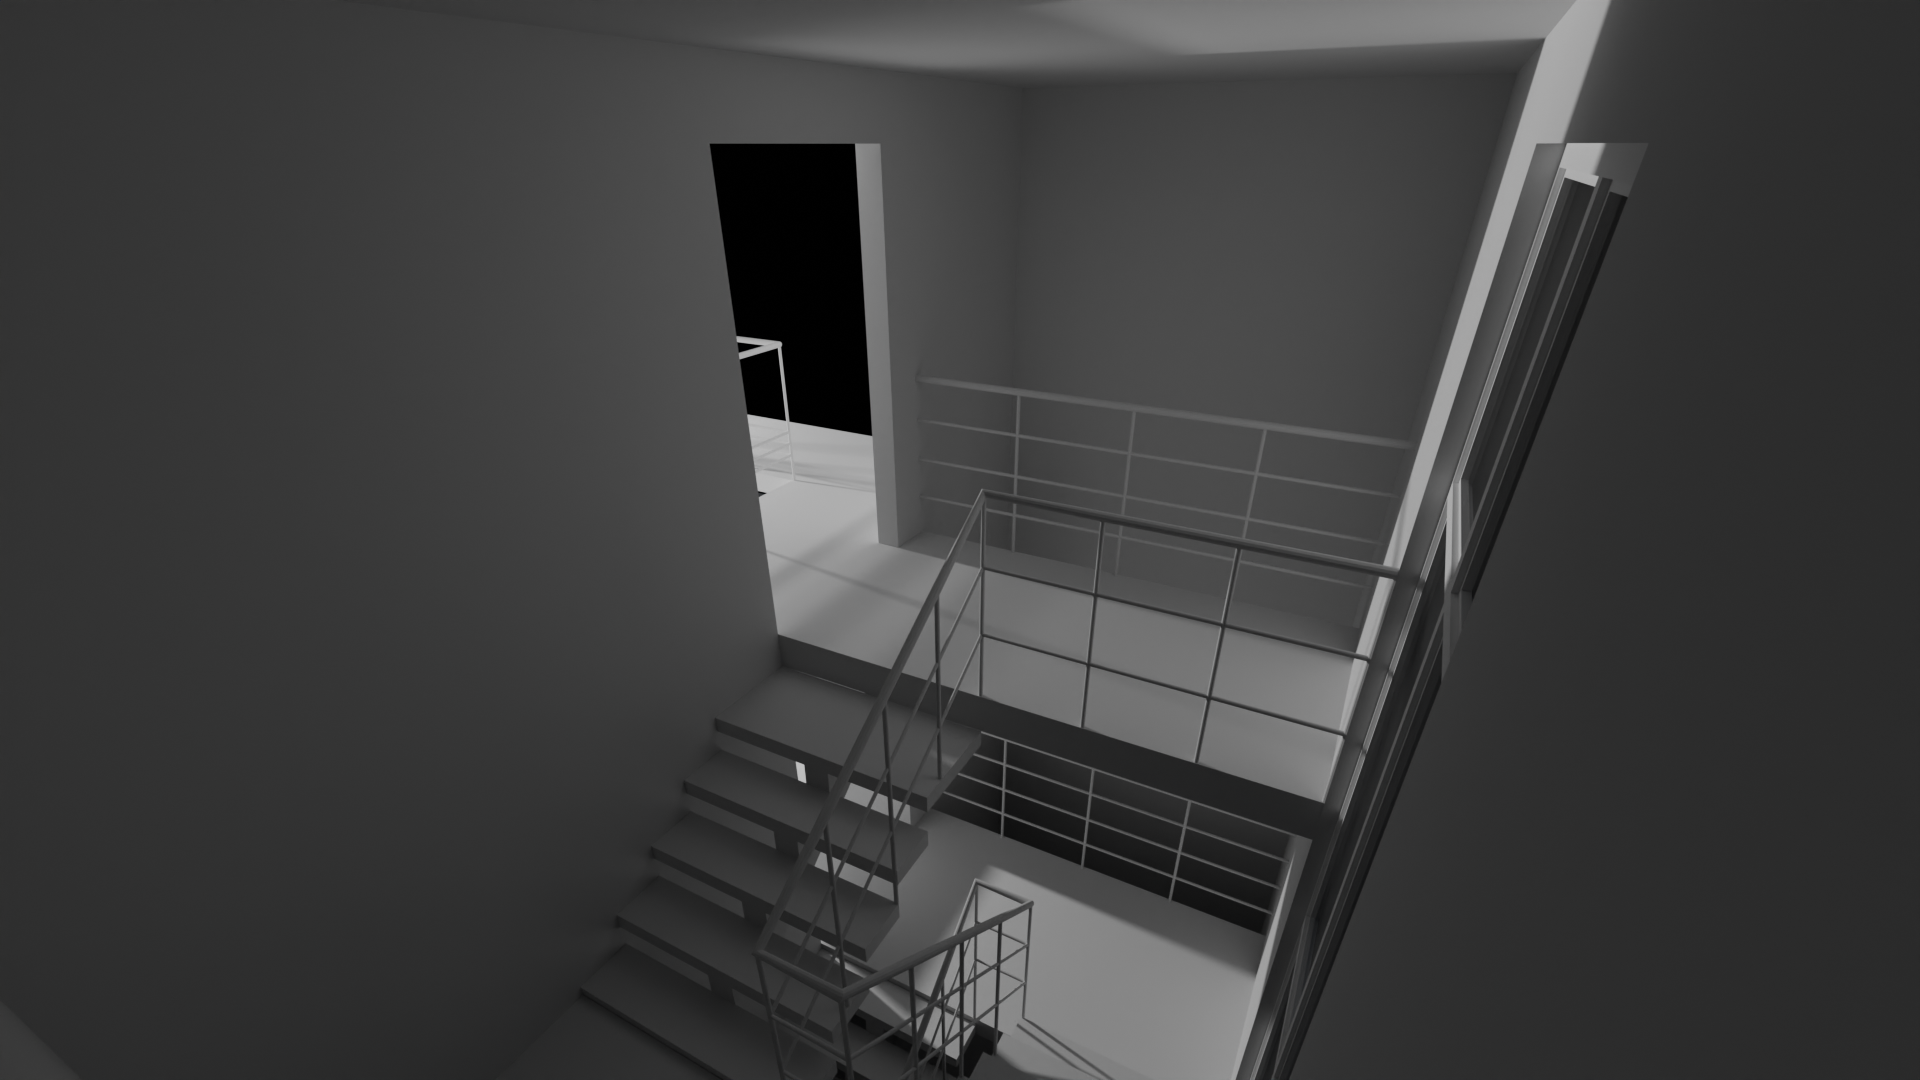
\includegraphics[width=0.5\textwidth]{./src/assets/untitled.png}
\caption{Exemplo de Figura}
\label{fig:exemplo}
\end{figure}

\begin{table}[ht]
\centering
\begin{tabular}{|c|c|c|}
\hline
Coluna 1 & Coluna 2 & Coluna 3 \\ \hline
Item 1   & Item 2   & Item 3   \\ \hline
Item 4   & Item 5   & Item 6   \\ \hline
\end{tabular}
\caption{Exemplo de Tabela}
\label{tab:exemplo}
\end{table}

\chapter{Conclusão}
\lipsum[11-12]

\bibliography{referencias}

\end{document}